%%% The main file. It contains definitions of basic parameters and includes all other parts.

%% Settings for single-side (simplex) printing
% Margins: left 40mm, right 25mm, top and bottom 25mm
% (but beware, LaTeX adds 1in implicitly)
\documentclass[12pt,a4paper]{report}
\setlength\textwidth{145mm}
\setlength\textheight{247mm}
\setlength\oddsidemargin{15mm}
\setlength\evensidemargin{15mm}
\setlength\topmargin{0mm}
\setlength\headsep{0mm}
\setlength\headheight{0mm}
% \openright makes the following text appear on a right-hand page
\let\openright=\clearpage

%% Settings for two-sided (duplex) printing
% \documentclass[12pt,a4paper,twoside,openright]{report}
% \setlength\textwidth{145mm}
% \setlength\textheight{247mm}
% \setlength\oddsidemargin{14.2mm}
% \setlength\evensidemargin{0mm}
% \setlength\topmargin{0mm}
% \setlength\headsep{0mm}
% \setlength\headheight{0mm}
% \let\openright=\cleardoublepage

%% Generate PDF/A-2u
\usepackage[a-2u]{pdfx}

%% Character encoding: usually latin2, cp1250 or utf8:
\usepackage[utf8]{inputenc}

%% Prefer Latin Modern fonts
\usepackage{lmodern}

%% Further useful packages (included in most LaTeX distributions)
\usepackage{amsmath}        % extensions for typesetting of math
\usepackage{amsfonts}       % math fonts
\usepackage{amsthm}         % theorems, definitions, etc.
\usepackage{bbding}         % various symbols (squares, asterisks, scissors, ...)
\usepackage{bm}             % boldface symbols (\bm)
\usepackage{graphicx}       % embedding of pictures
\usepackage{fancyvrb}       % improved verbatim environment
\usepackage{natbib}         % citation style AUTHOR (YEAR), or AUTHOR [NUMBER]
\usepackage[nottoc]{tocbibind} % makes sure that bibliography and the lists
			    % of figures/tables are included in the table
			    % of contents
\usepackage{dcolumn}        % improved alignment of table columns
\usepackage{booktabs}       % improved horizontal lines in tables
\usepackage{paralist}       % improved enumerate and itemize
\usepackage{xcolor}         % typesetting in color

\usepackage{listings}
\usepackage{enumitem}

\usepackage{hyperref}


\usepackage{color}
\definecolor{bluekeywords}{rgb}{0,0,1}
\definecolor{classgreen}{rgb}{0.17,0.57,0.68}
\definecolor{greencomments}{rgb}{0,0.5,0}
\definecolor{redstrings}{rgb}{0.64,0.08,0.08}
\definecolor{black}{rgb}{0,0,0}
\definecolor{blueattributes}{rgb}{0.37,0.52,0.62}
\definecolor{interfaceyellow}{rgb}{0.60,0.66,0.11}

\lstdefinestyle{cuda} {
	language=C++,
	commentstyle=\color{greencomments},
	stringstyle=\color{redstrings}\ttfamily, 
	keywordstyle=\color{bluekeywords},
%	morekeywords={  },
	emphstyle=[1]{\color{classgreen}},
	emphstyle=[2]{\color{interfaceyellow}}
}

\lstset{	
	captionpos=b,
	%numbers=left,
	%numberstyle=\tiny,
	columns=flexible,
	frame=single, 
	showspaces=false,
	showtabs=false,
	breaklines=true,
	showstringspaces=false,
	breakatwhitespace=true,
	escapeinside={(*@}{@*)},
	basicstyle=\ttfamily,
	tabsize=2
}

\graphicspath{ {./img/} }

%%% Basic information on the thesis

% Thesis title in English (exactly as in the formal assignment)
\def\ThesisTitle{Accelerating cross-correlation with GPUs}

% Author of the thesis
\def\ThesisAuthor{Karel Maděra}

% Year when the thesis is submitted
\def\YearSubmitted{2022}

% Name of the department or institute, where the work was officially assigned
% (according to the Organizational Structure of MFF UK in English,
% or a full name of a department outside MFF)
\def\Department{Name of the department}

% Is it a department (katedra), or an institute (ústav)?
\def\DeptType{Department}

% Thesis supervisor: name, surname and titles
\def\Supervisor{Supervisor's Name}

% Supervisor's department (again according to Organizational structure of MFF)
\def\SupervisorsDepartment{department}

% Study programme and specialization
\def\StudyProgramme{Computer Science}
\def\StudyBranch{ISS}

% An optional dedication: you can thank whomever you wish (your supervisor,
% consultant, a person who lent the software, etc.)
\def\Dedication{%
Dedication.
}

% Abstract (recommended length around 80-200 words; this is not a copy of your thesis assignment!)
\def\Abstract{%
Abstract.
}

% 3 to 5 keywords (recommended), each enclosed in curly braces
\def\Keywords{%
{key} {words}
}

%% The hyperref package for clickable links in PDF and also for storing
%% metadata to PDF (including the table of contents).
%% Most settings are pre-set by the pdfx package.
\hypersetup{unicode}
\hypersetup{breaklinks=true}
% PDF metadata
% https://tex.stackexchange.com/questions/26529/how-can-i-generate-pdf-metadata-from-latex
\hypersetup{
	pdftitle={\ThesisTitle},
	pdfauthor={\ThesisAuthor},
	pdfkeywords={\Keywords},
}
% Definitions of macros (see description inside)
%%% This file contains definitions of various useful macros and environments %%%
%%% Please add more macros here instead of cluttering other files with them. %%%

%%% Minor tweaks of style

% These macros employ a little dirty trick to convince LaTeX to typeset
% chapter headings sanely, without lots of empty space above them.
% Feel free to ignore.
\makeatletter
\def\@makechapterhead#1{
  {\parindent \z@ \raggedright \normalfont
   \Huge\bfseries \thechapter. #1
   \par\nobreak
   \vskip 20\p@
}}
\def\@makeschapterhead#1{
  {\parindent \z@ \raggedright \normalfont
   \Huge\bfseries #1
   \par\nobreak
   \vskip 20\p@
}}
\makeatother

% This macro defines a chapter, which is not numbered, but is included
% in the table of contents.
\def\chapwithtoc#1{
\chapter*{#1}
\addcontentsline{toc}{chapter}{#1}
}

% Draw black "slugs" whenever a line overflows, so that we can spot it easily.
\overfullrule=1mm

%%% Macros for definitions, theorems, claims, examples, ... (requires amsthm package)

\theoremstyle{plain}
\newtheorem{thm}{Theorem}
\newtheorem{lemma}[thm]{Lemma}
\newtheorem{claim}[thm]{Claim}

\theoremstyle{plain}
\newtheorem{defn}{Definition}

\theoremstyle{remark}
\newtheorem*{cor}{Corollary}
\newtheorem*{rem}{Remark}
\newtheorem*{example}{Example}

%%% An environment for proofs

\newenvironment{myproof}{
  \par\medskip\noindent
  \textit{Proof}.
}{
\newline
\rightline{$\qedsymbol$}
}

%%% An environment for typesetting of program code and input/output
%%% of programs. (Requires the fancyvrb package -- fancy verbatim.)

\DefineVerbatimEnvironment{code}{Verbatim}{fontsize=\small, frame=single}

%%% The field of all real and natural numbers
\newcommand{\R}{\mathbb{R}}
\newcommand{\N}{\mathbb{N}}

%%% Useful operators for statistics and probability
\DeclareMathOperator{\pr}{\textsf{P}}
\DeclareMathOperator{\E}{\textsf{E}\,}
\DeclareMathOperator{\var}{\textrm{var}}
\DeclareMathOperator{\sd}{\textrm{sd}}

%%% Transposition of a vector/matrix
\newcommand{\T}[1]{#1^\top}

%%% Various math goodies
\newcommand{\goto}{\rightarrow}
\newcommand{\gotop}{\stackrel{P}{\longrightarrow}}
\newcommand{\maon}[1]{o(n^{#1})}
\newcommand{\abs}[1]{\left|{#1}\right|}
\newcommand{\dint}{\int_0^\tau\!\!\int_0^\tau}
\newcommand{\isqr}[1]{\frac{1}{\sqrt{#1}}}

%%% Various table goodies
\newcommand{\pulrad}[1]{\raisebox{1.5ex}[0pt]{#1}}
\newcommand{\mc}[1]{\multicolumn{1}{c}{#1}}


% Title page and various mandatory informational pages
\begin{document}
%%% Title page of the thesis and other mandatory pages

%%% Title page of the thesis

\pagestyle{empty}
\hypersetup{pageanchor=false}
\begin{center}

\centerline{\mbox{
\includegraphics[width=166mm]{../img/logo-en.pdf}}}

\vspace{-8mm}
\vfill

{\bf\Large MASTER THESIS}

\vfill

{\LARGE\ThesisAuthor}

\vspace{15mm}

{\LARGE\bfseries\ThesisTitle}

\vfill

\Department

\vfill

{
\centerline{\vbox{\halign{\hbox to 0.45\hsize{\hfil #}&\hskip 0.5em\parbox[t]{0.45\hsize}{\raggedright #}\cr
Supervisor of the master thesis:&\Supervisor \cr
\noalign{\vspace{2mm}}
Study programme:&\StudyProgramme \cr
\noalign{\vspace{2mm}}
Study branch:&\StudyBranch \cr
}}}}

\vfill

% Zde doplňte rok
Prague \YearSubmitted

\end{center}

\newpage

%%% Here should be a bound sheet included -- a signed copy of the "master
%%% thesis assignment". This assignment is NOT a part of the electronic
%%% version of the thesis. DO NOT SCAN.

%%% A page with a solemn declaration to the master thesis

\openright
\hypersetup{pageanchor=true}
\pagestyle{plain}
\pagenumbering{roman}
\vglue 0pt plus 1fill

\noindent
I declare that I carried out this master thesis independently, and only with the cited
sources, literature and other professional sources. It has not been used to obtain another
or the same degree.

\medskip\noindent
I understand that my work relates to the rights and obligations under the Act No.~121/2000 Sb.,
the Copyright Act, as amended, in particular the fact that the Charles
University has the right to conclude a license agreement on the use of this
work as a school work pursuant to Section 60 subsection 1 of the Copyright~Act.

\vspace{10mm}

\hbox{\hbox to 0.5\hsize{%
In \hbox to 6em{\dotfill} date \hbox to 6em{\dotfill}
\hss}\hbox to 0.5\hsize{\dotfill\quad}}
\smallskip
\hbox{\hbox to 0.5\hsize{}\hbox to 0.5\hsize{\hfil Author's signature\hfil}}

\vspace{20mm}
\newpage

%%% Dedication

\openright

\noindent
\Dedication

\newpage

%%% Mandatory information page of the thesis

\openright

\vbox to 0.5\vsize{
\setlength\parindent{0mm}
\setlength\parskip{5mm}

Title:
\ThesisTitle

Author:
\ThesisAuthor

\DeptType:
\Department

Supervisor:
\Supervisor, \SupervisorsDepartment

Abstract:
\Abstract

Keywords:
\Keywords

\vss}

\newpage

\openright
\pagestyle{plain}
\pagenumbering{arabic}
\setcounter{page}{1}


%%% A page with automatically generated table of contents of the master thesis

\tableofcontents

%%% Each chapter is kept in a separate file
\chapter*{Introduction}
\addcontentsline{toc}{chapter}{Introduction}

The field of Signal processing is present everywhere in the today's world. From image processing through seismology to particle physics, the need to analyze, modify or synthesize signals such as sound, images and other scientific measurements is shared throughout many fields. One of the commonly used algorithms in signal processing is cross-correlation, which will be the subject of this thesis. The aim is to analyze, implement and evaluate possible methods of optimization and parallelization of definition based cross-correlation algorithm. The implementations will then be further compared to the generally used implementation based on Fast Fourier transform.

\section*{Motivation}

Cross-correlation is one of the key operations in both analog and digital signal processing.
It is widely used in image analysis, pattern recognition, image segmentation, particle physics, electron tomography, and many other fields \citep{Kapinchev2015}. For many of these applications, the computational complexity of cross-corellation is often the limiting factor in the data processing pipeline. The amount of input data combined with the computational complexity make simple sequential CPU-based implementations and even more advanced parallel CPU-based implementation inadequate.

Algorithms based on the definition of cross-correlation or on Fast Fourier transform (FFT) can take advantage of the inherent high degree of data parallelism in the definition of cross-correlation or FFT respectively to utilize the high throughput and massive amounts of computational power provided by massively parallel systems in the form of Graphical processing units (GPU).

This thesis is a continuation of the thesis "Employing GPU to Process Data from Electron Microscope" \citep{misko}, which uses both basic definition based cross-corellation as well as one based on FFT. This thesis aims to compare the asymptotically faster FFT based algorithm with the asymptotically slower definition based algorithm and provide an optimized implementation of the definition based algorithm which, for the input sizes used by the original thesis, will be faster than the FFT based implementation.

\section*{Goals}
The goal of this thesis is to analyze the possibilities for optimization and parallelization of the definition based algorithm and provide detailed measurements and comparisons with the FFT based algorithm for range of input forms and sizes. The optimizations and parallelization of the definition based algorithm will utilize capabilities provided by the CUDA platform.

In steps, this thesis will:
\begin{itemize}
	\item analyze optimizations of the definition based algorithm, focused on parallelization using CUDA platform,
	\item compare the optimized implementations with one based on Fast Fourier transform,
	\item measure different input sizes and types for both the optimized definition based and Fast Fourier transform based algorithms
\end{itemize}





\chapter{Cross-correlation}
\label{sec:cross-corr}
%\addcontentsline{toc}{chapter}{Cross-correlation}

% TODO: Cite wikipedia or find some other introduction
In this chapter, we define cross-correlation and its variants. We first define one-dimensional cross-correlation, extending it into multiple dimensions and introducing periodic and circular cross-correlation. We then describe how these variations are used to compute cross-correlation using Fast Fourier transform. Lastly we describe the possibilities for optimization and parallelization of cross-correlation, with real-world usage examples where these optimizations could be used.
% TODO: Maybe mention different data layouts such as one_to_one, one_to_many etc.


\section{Definition}

Cross-correlation, also known as sliding dot product or sliding inner-product, is a function describing similarity of two series or two functions based on their relative displacement \citep{site:wiki_cross_corr}.
Cross-correlation of functions $f,g: \mathbb{C} \rightarrow \mathbb{R}$, denoted as \(f \star g\), is defined by the following formula:
\[
	(f \star g)(\tau) = \int_{-\infty}^{\infty} \overline{f(t)}g(t + \tau) \,dt,
\] 

where \(\overline{f(t)}\) denotes the complex conjugate of \(f(t)\) and \(\tau\) is the displacement of the two functions \(f\) and \(g\). In simpler words, the value \((f \star g)(\tau)\) tells us how similar the function \(f\) is to \(g\) when \(g\) is shifted by \(\tau\), with higher value representing higher similarity. Figure \ref{fig:cross_corr_example} shows cross-correlation of two example functions.

\begin{figure}[h]
	\centering
	\def\svgwidth{0.8\textwidth}
	% Must be relative to current directory
	% as input ignores graphicspath, which is
	% only for includegraphics{}
	
\chapter{Cross-correlation}
\label{sec:cross-corr}
%\addcontentsline{toc}{chapter}{Cross-correlation}

% TODO: Cite wikipedia or find some other introduction
In this chapter, we define cross-correlation and its variants. We first define one-dimensional cross-correlation, extending it into multiple dimensions and introducing periodic and circular cross-correlation. We then describe how these variations are used to compute cross-correlation using Fast Fourier transform. Lastly we describe the possibilities for optimization and parallelization of cross-correlation, with real-world usage examples where these optimizations could be used.
% TODO: Maybe mention different data layouts such as one_to_one, one_to_many etc.


\section{Definition}

Cross-correlation, also known as sliding dot product or sliding inner-product, is a function describing similarity of two series or two functions based on their relative displacement \citep{site:wiki_cross_corr}.
Cross-correlation of functions $f,g: \mathbb{C} \rightarrow \mathbb{R}$, denoted as \(f \star g\), is defined by the following formula:
\[
	(f \star g)(\tau) = \int_{-\infty}^{\infty} \overline{f(t)}g(t + \tau) \,dt,
\] 

where \(\overline{f(t)}\) denotes the complex conjugate of \(f(t)\) and \(\tau\) is the displacement of the two functions \(f\) and \(g\). In simpler words, the value \((f \star g)(\tau)\) tells us how similar the function \(f\) is to \(g\) when \(g\) is shifted by \(\tau\), with higher value representing higher similarity. Figure \ref{fig:cross_corr_example} shows cross-correlation of two example functions.

\begin{figure}[h]
	\centering
	\def\svgwidth{0.8\textwidth}
	% Must be relative to current directory
	% as input ignores graphicspath, which is
	% only for includegraphics{}
	
\chapter{Cross-correlation}
\label{sec:cross-corr}
%\addcontentsline{toc}{chapter}{Cross-correlation}

% TODO: Cite wikipedia or find some other introduction
In this chapter, we define cross-correlation and its variants. We first define one-dimensional cross-correlation, extending it into multiple dimensions and introducing periodic and circular cross-correlation. We then describe how these variations are used to compute cross-correlation using Fast Fourier transform. Lastly we describe the possibilities for optimization and parallelization of cross-correlation, with real-world usage examples where these optimizations could be used.
% TODO: Maybe mention different data layouts such as one_to_one, one_to_many etc.


\section{Definition}

Cross-correlation, also known as sliding dot product or sliding inner-product, is a function describing similarity of two series or two functions based on their relative displacement \citep{site:wiki_cross_corr}.
Cross-correlation of functions $f,g: \mathbb{C} \rightarrow \mathbb{R}$, denoted as \(f \star g\), is defined by the following formula:
\[
	(f \star g)(\tau) = \int_{-\infty}^{\infty} \overline{f(t)}g(t + \tau) \,dt,
\] 

where \(\overline{f(t)}\) denotes the complex conjugate of \(f(t)\) and \(\tau\) is the displacement of the two functions \(f\) and \(g\). In simpler words, the value \((f \star g)(\tau)\) tells us how similar the function \(f\) is to \(g\) when \(g\) is shifted by \(\tau\), with higher value representing higher similarity. Figure \ref{fig:cross_corr_example} shows cross-correlation of two example functions.

\begin{figure}[h]
	\centering
	\def\svgwidth{0.8\textwidth}
	% Must be relative to current directory
	% as input ignores graphicspath, which is
	% only for includegraphics{}
	\input{./img/crosscorr.pdf_tex}
	\caption{Cross-correlation of two functions. \cite{pic:crosscorr}}
	\label{fig:cross_corr_example}
\end{figure}

For two discrete functions, as will be used in our case, cross-correlation of functions \( f, g : \mathbb{Z} \rightarrow \mathbb{R} \) is defined by the following formula:

\[
(f \star g)[m] = \sum_{i=-\infty}^{\infty} \overline{f[i]}g[i + m],
\] 



This definition of cross-correlation can be extended for use in two dimensions, as is required, for example, in image processing.
For two discrete functions \( f, g : \mathbb{Z}^2 \rightarrow \mathbb{R} \), cross-correlation is defined as:

\[
(f \star g)[m,n] = \sum_{i=-\infty}^{\infty} \sum_{j=-\infty}^{\infty} \overline{f[m,n]}g[m + i,n + j],
\]

Even though cross-correlation is defined on the whole $\mathbb{Z}$ for one dimension and $\mathbb{Z}^2$ for two dimensions, most use cases of cross-correlation work only on finite inputs, such as image processing working on finite images. The only values we are interested in are when the two images overlap, which limits the computation to $(w_1 + w_2 - 1) * (h_1 + h_2 - 1)$, where $w_i$ denotes width of the image $i$ and $h_i$ denotes the height of the image $i$.

This limits the part of the output we are interested in and leads us to time complexity of the definition based algorithm, or \textit{naive} algorithm as it is called in the code associated with the thesis. For each of the $(w_1 + w_2 - 1) * (h_1 + h_2 - 1)$ output values, we need to multiply the overlapping pixel values and sum all the multiplication results together. There will be at most $min(w_1, w_2) * min(h_1, h_2)$ overlapping pixels. For simplicity, let us work with two images of size $w_i*h_i$. Then the time complexity of the definition based algorithm is $((2*w_i-1)*(2 * h_i - 1) * (w_i * h_i))$, which gives us asymptotic complexity of $\mathcal{O}(w_i^2*h_i^2)$.

\section{Computation using discrete Fourier Transform}
\label{sec:cross_corr_fft}

In this section, we describe an algorithm which uses discrete Fourier transform to compute cross-correlation of two finite two-dimensional series. The asymptotic complexity of this algorithm will be $\mathcal{O}(w_i*h_i*\log_2(w_i*h_i))$, where $w_i$ is the width of each series and $h_i$ the height of each series. This improves on the asymptotic complexity $\mathcal{O}(w_i^2*h_i^2)$ of the definition based algorithm described in the previous section \ref{sec:cross-corr}.

Discrete Fourier transform can only be used to compute a special type of cross-correlation, so called \textit{circular} cross-correlation.
For finite series $N \in \mathbb{N} \{x\}_n = x_0, x_1, ..., x_{N-1}, \{y_n\} = y_0, y_1, ..., y_{N-1}$, circular cross-correlation is defined as:

\[
(x \star_N y)_m = \sum_{i=0}^{N-1} \overline{x_m} y_{(m + i) mod N},
\]

where $\overline{x_m}$ denotes complex conjugate of $x_m$.


Based on the Cross-Correlation Theorem \citep{thesis:wang}, circular cross-correlation $(x \star_N y)_m$ can be computed using discrete Fourier Transform based on the following formula:

\[
(x \star_N y)_m = \mathbb{F}^{-1}(\overline{\mathbb{F}(x)}*\mathbb{F}(y))
\]

where $\mathbb{F}(x)$ and $\mathbb{F}(y)$ denote discrete Fourier Transform of series $x$ and $y$ respectively, $\overline{\mathbb{F}(x)}$ denotes complex conjugate of the discrete Fourier Transform, $*$ denotes element-wise multiplication of two series and $\mathbb{F}^{-1}$ denotes inverse discrete Fourier Transform.

For two series $\{x_n\}$ and $\{y_n\}$, we would thus first compute their discrete Fourier transforms $\{X_n\}$ and $\{Y_n\}$. Then we would compute the complex conjugate $\overline{X}$ of $\{X_n\}$, multiply the corresponding elements of $\overline{X}$ and $\{Y_n\}$ and finally compute the inverse Fourier transform of the result. The time complexity of this algorithm is $\mathcal{O}(N\log(N))$ for the Fourier transform, $\mathcal{O}(N)$ for complex conjugate, $\mathcal{O}(N)$ for element-wise multiplication and $\mathcal{O}(N\log(N))$ for inverse Fourier transform. This gives us the resulting resulting asymptotic time complexity of $\mathcal{O}(N\log(N))$.


Circular cross-correlation can be imagined as a cross-correlation of two periodic discrete functions. When computing circular cross-correlation by definition, for each shift the last element shifted off the series end is taken from the back and moved to the front. This is the circular shift done by the modulo operator. If we assume infinite periodic functions, circular shift is equivalent to linear shift, as the first element is first in each period. If we then compute the sum from linear cross-correlation only over a single period, we can see that the result is equivalent to circular cross-correlation of the two functions.
% TODO: Cite https://inst.eecs.berkeley.edu/~ee16a/fa18/lectures/Note22.pdf

We call this the periodic cross-correlation, for finite series $n \in \mathbb{N} \{x\}_n = x_0, x_1, ..., x_{n-1}, \{y_n\} = y_0, y_1, ..., y_{n-1} \in \mathbb{C}^N$ defined as:

\[
(x \star_pN y)_m = \sum_{i=0}^{N-1} \overline{x_m} y_{(m + i)},
\]


To calculate linear (non-circular) cross-correlation of finite series using circular cross-correlation, we observe the following equality.



Compared to non-periodic linear cross-correlation, periodic linear cross-correlation is summed only over the length of the period, and is thus equivalent to a linear cross-correlation of one period zero extended to infinity.

If we observe the corresponding linear shift in periodic linear cross-correlation, we can observe on Figure \ref{fig:circular_cross_corr} that the multiplied values for each shift are the same in both computations. Thus the results are the same for both when computing linear cross-correlation only over the length of the period.

% TODO: Illustrative Image
Thus if we zero extend the series to twice its length and compute the circular cross-correlation of this series, the result is the same as linear cross-correlation of the original series zero extended to infinity.

% TODO: Circular shift

% TODO: Expand this
The same equivalence holds for two-dimensional linear and circular cross-correlations as well. 

% TODO: Modify this

% TODO: Expand the circular shift
Result is a matrix $z \in \mathbb{R}^2$ of size $2w*2h$ with the result of cross-correlation in the bottom right quadrant.

\section{Parallelization and optimizations}
In the original thesis by \citep{misko}, and in the field of image processing in general, 2D version of cross-correlation is mostly used to find a grayscale image or a piece of a grayscale image represented as integer matrix in another image. This can be done to for example find a displacement of a certain point of interest between images of one item taken at different times, as is done in \citet{misko} and \citet{zhang2015}. 

This thesis will implement cross-correlation of integer and floating point matrices, which is more general and can be used in works mentioned above. The implementations will be optimized to take advantage of different forms of cross-correlation input, such as cross-correlation of one matrix with many other matrices, different sizes of input matrices etc. 
% TODO: Expand

\subsection{Forms of cross-correlation}

In works using cross-correlation, there are several forms of computation which can be used for optimization such as data caching and reuse, batching, precomputing etc. The forms differ in the number of inputs and in the way cross-correlation is computed between different inputs. 
The two basic forms are:

\begin{enumerate}
	\item n left inputs, each with m different right inputs (n to mn) \citet{misko} \citet{zhang2015} \citet{Kapinchev2015}, 
	\item x left inputs, each with all y right different inputs (n to m) \citet{Clark2011}.
\end{enumerate} 

There are several subtypes which can also be optimized for. For \textit{n} left inputs with disjoint sets of \textit{m} right inputs for each of the left inputs, we have the following subtypes:

\begin{enumerate}
	\item one to one,
	\item one to many,
	\item large number of pairs.
\end{enumerate}

With these subtypes, we can more aggressively cache and reuse the left input. Any implementation capable of processing the general input form can also be used to implement all of these subtypes.
% We use this with the warp shuffle and warp shift implementations
Inversely, optimized implementation of the any of the above subtypes can be used to implement the general n to mn input type and transitively any of the other subtypes.

Any implementation of the \textit{one to many} subtype can also be used to implement the other major type, the \textit{x to y} type, by running the \textit{one to many} \textit{x} times, possibly in parallel.


%The following are examples of cross-correlation usage:
%\begin{itemize}
%	\item \citet{misko} computes cross-correlation between multiple subregions of a reference image with the corresponding subregion in multiple deformed images.
%	\item \citet{zhang2015} differs from \citep{misko} only in a processing that follows the cross-correlation phase which is outside the scope of this thesis.
%	\item \citet{Kapinchev2015} computes cross-correlation of one input signal with a number of masks to determine the values for all depths in parallel. The presented implementation does cross-correlation with each mask separately, computing them sequentially one after another, but this is due to the memory limitations of hardware and the optimal solution would be to compute the cross-correlation of the input signal with all masks in parallel.
%	\item \citet{Clark2011} computes cross-correlation of time series, where signal from each antenna with the signal from all other antennas.
	% TODO: Additional usecases
%\end{itemize}


\subsection{Post-processing}

In most use cases, cross-correlation itself is not a final output but the results are used further in further processing.

It is often used to find position of a smaller signal in larger signal, for example in the field of Digital image processing for template matching, image alignment etc. In these use cases, the only information of interest is the maximum value in the result matrix. 

In Digital Image correlation, we are also interested in finding the maximum, but this time with a subpixel precision. This requires us to find the maximum value and use the results in an area around it to interpolate a function \citep{zhang2015} \citep{misko}.

In the field of Seismology, cross-correlation is used for picking, ambient noise monitoring, waveform comparison and signal, event and pattern detection. \citep{Ventosa2019}
 
In optical coherence tomography, the whole result of cross-correlation summed to compute the intensity of each pixel \citep{Kapinchev2015}. 

Any post-processing is outside of the scope of this thesis. Result of cross-correlation will be taken as-is and validated against preexisting cross-correlation implementations.
% TODO: Go through the examples and see what they do with the results

% TODO: Post processing, what is the usual output etc.
% TODO: Menion that we are not doing any postprocessing


	\caption{Cross-correlation of two functions. \cite{pic:crosscorr}}
	\label{fig:cross_corr_example}
\end{figure}

For two discrete functions, as will be used in our case, cross-correlation of functions \( f, g : \mathbb{Z} \rightarrow \mathbb{R} \) is defined by the following formula:

\[
(f \star g)[m] = \sum_{i=-\infty}^{\infty} \overline{f[i]}g[i + m],
\] 



This definition of cross-correlation can be extended for use in two dimensions, as is required, for example, in image processing.
For two discrete functions \( f, g : \mathbb{Z}^2 \rightarrow \mathbb{R} \), cross-correlation is defined as:

\[
(f \star g)[m,n] = \sum_{i=-\infty}^{\infty} \sum_{j=-\infty}^{\infty} \overline{f[m,n]}g[m + i,n + j],
\]

Even though cross-correlation is defined on the whole $\mathbb{Z}$ for one dimension and $\mathbb{Z}^2$ for two dimensions, most use cases of cross-correlation work only on finite inputs, such as image processing working on finite images. The only values we are interested in are when the two images overlap, which limits the computation to $(w_1 + w_2 - 1) * (h_1 + h_2 - 1)$, where $w_i$ denotes width of the image $i$ and $h_i$ denotes the height of the image $i$.

This limits the part of the output we are interested in and leads us to time complexity of the definition based algorithm, or \textit{naive} algorithm as it is called in the code associated with the thesis. For each of the $(w_1 + w_2 - 1) * (h_1 + h_2 - 1)$ output values, we need to multiply the overlapping pixel values and sum all the multiplication results together. There will be at most $min(w_1, w_2) * min(h_1, h_2)$ overlapping pixels. For simplicity, let us work with two images of size $w_i*h_i$. Then the time complexity of the definition based algorithm is $((2*w_i-1)*(2 * h_i - 1) * (w_i * h_i))$, which gives us asymptotic complexity of $\mathcal{O}(w_i^2*h_i^2)$.

\section{Computation using discrete Fourier Transform}
\label{sec:cross_corr_fft}

In this section, we describe an algorithm which uses discrete Fourier transform to compute cross-correlation of two finite two-dimensional series. The asymptotic complexity of this algorithm will be $\mathcal{O}(w_i*h_i*\log_2(w_i*h_i))$, where $w_i$ is the width of each series and $h_i$ the height of each series. This improves on the asymptotic complexity $\mathcal{O}(w_i^2*h_i^2)$ of the definition based algorithm described in the previous section \ref{sec:cross-corr}.

Discrete Fourier transform can only be used to compute a special type of cross-correlation, so called \textit{circular} cross-correlation.
For finite series $N \in \mathbb{N} \{x\}_n = x_0, x_1, ..., x_{N-1}, \{y_n\} = y_0, y_1, ..., y_{N-1}$, circular cross-correlation is defined as:

\[
(x \star_N y)_m = \sum_{i=0}^{N-1} \overline{x_m} y_{(m + i) mod N},
\]

where $\overline{x_m}$ denotes complex conjugate of $x_m$.


Based on the Cross-Correlation Theorem \citep{thesis:wang}, circular cross-correlation $(x \star_N y)_m$ can be computed using discrete Fourier Transform based on the following formula:

\[
(x \star_N y)_m = \mathbb{F}^{-1}(\overline{\mathbb{F}(x)}*\mathbb{F}(y))
\]

where $\mathbb{F}(x)$ and $\mathbb{F}(y)$ denote discrete Fourier Transform of series $x$ and $y$ respectively, $\overline{\mathbb{F}(x)}$ denotes complex conjugate of the discrete Fourier Transform, $*$ denotes element-wise multiplication of two series and $\mathbb{F}^{-1}$ denotes inverse discrete Fourier Transform.

For two series $\{x_n\}$ and $\{y_n\}$, we would thus first compute their discrete Fourier transforms $\{X_n\}$ and $\{Y_n\}$. Then we would compute the complex conjugate $\overline{X}$ of $\{X_n\}$, multiply the corresponding elements of $\overline{X}$ and $\{Y_n\}$ and finally compute the inverse Fourier transform of the result. The time complexity of this algorithm is $\mathcal{O}(N\log(N))$ for the Fourier transform, $\mathcal{O}(N)$ for complex conjugate, $\mathcal{O}(N)$ for element-wise multiplication and $\mathcal{O}(N\log(N))$ for inverse Fourier transform. This gives us the resulting resulting asymptotic time complexity of $\mathcal{O}(N\log(N))$.


Circular cross-correlation can be imagined as a cross-correlation of two periodic discrete functions. When computing circular cross-correlation by definition, for each shift the last element shifted off the series end is taken from the back and moved to the front. This is the circular shift done by the modulo operator. If we assume infinite periodic functions, circular shift is equivalent to linear shift, as the first element is first in each period. If we then compute the sum from linear cross-correlation only over a single period, we can see that the result is equivalent to circular cross-correlation of the two functions.
% TODO: Cite https://inst.eecs.berkeley.edu/~ee16a/fa18/lectures/Note22.pdf

We call this the periodic cross-correlation, for finite series $n \in \mathbb{N} \{x\}_n = x_0, x_1, ..., x_{n-1}, \{y_n\} = y_0, y_1, ..., y_{n-1} \in \mathbb{C}^N$ defined as:

\[
(x \star_pN y)_m = \sum_{i=0}^{N-1} \overline{x_m} y_{(m + i)},
\]


To calculate linear (non-circular) cross-correlation of finite series using circular cross-correlation, we observe the following equality.



Compared to non-periodic linear cross-correlation, periodic linear cross-correlation is summed only over the length of the period, and is thus equivalent to a linear cross-correlation of one period zero extended to infinity.

If we observe the corresponding linear shift in periodic linear cross-correlation, we can observe on Figure \ref{fig:circular_cross_corr} that the multiplied values for each shift are the same in both computations. Thus the results are the same for both when computing linear cross-correlation only over the length of the period.

% TODO: Illustrative Image
Thus if we zero extend the series to twice its length and compute the circular cross-correlation of this series, the result is the same as linear cross-correlation of the original series zero extended to infinity.

% TODO: Circular shift

% TODO: Expand this
The same equivalence holds for two-dimensional linear and circular cross-correlations as well. 

% TODO: Modify this

% TODO: Expand the circular shift
Result is a matrix $z \in \mathbb{R}^2$ of size $2w*2h$ with the result of cross-correlation in the bottom right quadrant.

\section{Parallelization and optimizations}
In the original thesis by \citep{misko}, and in the field of image processing in general, 2D version of cross-correlation is mostly used to find a grayscale image or a piece of a grayscale image represented as integer matrix in another image. This can be done to for example find a displacement of a certain point of interest between images of one item taken at different times, as is done in \citet{misko} and \citet{zhang2015}. 

This thesis will implement cross-correlation of integer and floating point matrices, which is more general and can be used in works mentioned above. The implementations will be optimized to take advantage of different forms of cross-correlation input, such as cross-correlation of one matrix with many other matrices, different sizes of input matrices etc. 
% TODO: Expand

\subsection{Forms of cross-correlation}

In works using cross-correlation, there are several forms of computation which can be used for optimization such as data caching and reuse, batching, precomputing etc. The forms differ in the number of inputs and in the way cross-correlation is computed between different inputs. 
The two basic forms are:

\begin{enumerate}
	\item n left inputs, each with m different right inputs (n to mn) \citet{misko} \citet{zhang2015} \citet{Kapinchev2015}, 
	\item x left inputs, each with all y right different inputs (n to m) \citet{Clark2011}.
\end{enumerate} 

There are several subtypes which can also be optimized for. For \textit{n} left inputs with disjoint sets of \textit{m} right inputs for each of the left inputs, we have the following subtypes:

\begin{enumerate}
	\item one to one,
	\item one to many,
	\item large number of pairs.
\end{enumerate}

With these subtypes, we can more aggressively cache and reuse the left input. Any implementation capable of processing the general input form can also be used to implement all of these subtypes.
% We use this with the warp shuffle and warp shift implementations
Inversely, optimized implementation of the any of the above subtypes can be used to implement the general n to mn input type and transitively any of the other subtypes.

Any implementation of the \textit{one to many} subtype can also be used to implement the other major type, the \textit{x to y} type, by running the \textit{one to many} \textit{x} times, possibly in parallel.


%The following are examples of cross-correlation usage:
%\begin{itemize}
%	\item \citet{misko} computes cross-correlation between multiple subregions of a reference image with the corresponding subregion in multiple deformed images.
%	\item \citet{zhang2015} differs from \citep{misko} only in a processing that follows the cross-correlation phase which is outside the scope of this thesis.
%	\item \citet{Kapinchev2015} computes cross-correlation of one input signal with a number of masks to determine the values for all depths in parallel. The presented implementation does cross-correlation with each mask separately, computing them sequentially one after another, but this is due to the memory limitations of hardware and the optimal solution would be to compute the cross-correlation of the input signal with all masks in parallel.
%	\item \citet{Clark2011} computes cross-correlation of time series, where signal from each antenna with the signal from all other antennas.
	% TODO: Additional usecases
%\end{itemize}


\subsection{Post-processing}

In most use cases, cross-correlation itself is not a final output but the results are used further in further processing.

It is often used to find position of a smaller signal in larger signal, for example in the field of Digital image processing for template matching, image alignment etc. In these use cases, the only information of interest is the maximum value in the result matrix. 

In Digital Image correlation, we are also interested in finding the maximum, but this time with a subpixel precision. This requires us to find the maximum value and use the results in an area around it to interpolate a function \citep{zhang2015} \citep{misko}.

In the field of Seismology, cross-correlation is used for picking, ambient noise monitoring, waveform comparison and signal, event and pattern detection. \citep{Ventosa2019}
 
In optical coherence tomography, the whole result of cross-correlation summed to compute the intensity of each pixel \citep{Kapinchev2015}. 

Any post-processing is outside of the scope of this thesis. Result of cross-correlation will be taken as-is and validated against preexisting cross-correlation implementations.
% TODO: Go through the examples and see what they do with the results

% TODO: Post processing, what is the usual output etc.
% TODO: Menion that we are not doing any postprocessing


	\caption{Cross-correlation of two functions. \cite{pic:crosscorr}}
	\label{fig:cross_corr_example}
\end{figure}

For two discrete functions, as will be used in our case, cross-correlation of functions \( f, g : \mathbb{Z} \rightarrow \mathbb{R} \) is defined by the following formula:

\[
(f \star g)[m] = \sum_{i=-\infty}^{\infty} \overline{f[i]}g[i + m],
\] 



This definition of cross-correlation can be extended for use in two dimensions, as is required, for example, in image processing.
For two discrete functions \( f, g : \mathbb{Z}^2 \rightarrow \mathbb{R} \), cross-correlation is defined as:

\[
(f \star g)[m,n] = \sum_{i=-\infty}^{\infty} \sum_{j=-\infty}^{\infty} \overline{f[m,n]}g[m + i,n + j],
\]

Even though cross-correlation is defined on the whole $\mathbb{Z}$ for one dimension and $\mathbb{Z}^2$ for two dimensions, most use cases of cross-correlation work only on finite inputs, such as image processing working on finite images. The only values we are interested in are when the two images overlap, which limits the computation to $(w_1 + w_2 - 1) * (h_1 + h_2 - 1)$, where $w_i$ denotes width of the image $i$ and $h_i$ denotes the height of the image $i$.

This limits the part of the output we are interested in and leads us to time complexity of the definition based algorithm, or \textit{naive} algorithm as it is called in the code associated with the thesis. For each of the $(w_1 + w_2 - 1) * (h_1 + h_2 - 1)$ output values, we need to multiply the overlapping pixel values and sum all the multiplication results together. There will be at most $min(w_1, w_2) * min(h_1, h_2)$ overlapping pixels. For simplicity, let us work with two images of size $w_i*h_i$. Then the time complexity of the definition based algorithm is $((2*w_i-1)*(2 * h_i - 1) * (w_i * h_i))$, which gives us asymptotic complexity of $\mathcal{O}(w_i^2*h_i^2)$.

\section{Computation using discrete Fourier Transform}
\label{sec:cross_corr_fft}

In this section, we describe an algorithm which uses discrete Fourier transform to compute cross-correlation of two finite two-dimensional series. The asymptotic complexity of this algorithm will be $\mathcal{O}(w_i*h_i*\log_2(w_i*h_i))$, where $w_i$ is the width of each series and $h_i$ the height of each series. This improves on the asymptotic complexity $\mathcal{O}(w_i^2*h_i^2)$ of the definition based algorithm described in the previous section \ref{sec:cross-corr}.

Discrete Fourier transform can only be used to compute a special type of cross-correlation, so called \textit{circular} cross-correlation.
For finite series $N \in \mathbb{N} \{x\}_n = x_0, x_1, ..., x_{N-1}, \{y_n\} = y_0, y_1, ..., y_{N-1}$, circular cross-correlation is defined as:

\[
(x \star_N y)_m = \sum_{i=0}^{N-1} \overline{x_m} y_{(m + i) mod N},
\]

where $\overline{x_m}$ denotes complex conjugate of $x_m$.


Based on the Cross-Correlation Theorem \citep{thesis:wang}, circular cross-correlation $(x \star_N y)_m$ can be computed using discrete Fourier Transform based on the following formula:

\[
(x \star_N y)_m = \mathbb{F}^{-1}(\overline{\mathbb{F}(x)}*\mathbb{F}(y))
\]

where $\mathbb{F}(x)$ and $\mathbb{F}(y)$ denote discrete Fourier Transform of series $x$ and $y$ respectively, $\overline{\mathbb{F}(x)}$ denotes complex conjugate of the discrete Fourier Transform, $*$ denotes element-wise multiplication of two series and $\mathbb{F}^{-1}$ denotes inverse discrete Fourier Transform.

For two series $\{x_n\}$ and $\{y_n\}$, we would thus first compute their discrete Fourier transforms $\{X_n\}$ and $\{Y_n\}$. Then we would compute the complex conjugate $\overline{X}$ of $\{X_n\}$, multiply the corresponding elements of $\overline{X}$ and $\{Y_n\}$ and finally compute the inverse Fourier transform of the result. The time complexity of this algorithm is $\mathcal{O}(N\log(N))$ for the Fourier transform, $\mathcal{O}(N)$ for complex conjugate, $\mathcal{O}(N)$ for element-wise multiplication and $\mathcal{O}(N\log(N))$ for inverse Fourier transform. This gives us the resulting resulting asymptotic time complexity of $\mathcal{O}(N\log(N))$.


Circular cross-correlation can be imagined as a cross-correlation of two periodic discrete functions. When computing circular cross-correlation by definition, for each shift the last element shifted off the series end is taken from the back and moved to the front. This is the circular shift done by the modulo operator. If we assume infinite periodic functions, circular shift is equivalent to linear shift, as the first element is first in each period. If we then compute the sum from linear cross-correlation only over a single period, we can see that the result is equivalent to circular cross-correlation of the two functions.
% TODO: Cite https://inst.eecs.berkeley.edu/~ee16a/fa18/lectures/Note22.pdf

We call this the periodic cross-correlation, for finite series $n \in \mathbb{N} \{x\}_n = x_0, x_1, ..., x_{n-1}, \{y_n\} = y_0, y_1, ..., y_{n-1} \in \mathbb{C}^N$ defined as:

\[
(x \star_pN y)_m = \sum_{i=0}^{N-1} \overline{x_m} y_{(m + i)},
\]


To calculate linear (non-circular) cross-correlation of finite series using circular cross-correlation, we observe the following equality.



Compared to non-periodic linear cross-correlation, periodic linear cross-correlation is summed only over the length of the period, and is thus equivalent to a linear cross-correlation of one period zero extended to infinity.

If we observe the corresponding linear shift in periodic linear cross-correlation, we can observe on Figure \ref{fig:circular_cross_corr} that the multiplied values for each shift are the same in both computations. Thus the results are the same for both when computing linear cross-correlation only over the length of the period.

% TODO: Illustrative Image
Thus if we zero extend the series to twice its length and compute the circular cross-correlation of this series, the result is the same as linear cross-correlation of the original series zero extended to infinity.

% TODO: Circular shift

% TODO: Expand this
The same equivalence holds for two-dimensional linear and circular cross-correlations as well. 

% TODO: Modify this

% TODO: Expand the circular shift
Result is a matrix $z \in \mathbb{R}^2$ of size $2w*2h$ with the result of cross-correlation in the bottom right quadrant.

\section{Parallelization and optimizations}
In the original thesis by \citep{misko}, and in the field of image processing in general, 2D version of cross-correlation is mostly used to find a grayscale image or a piece of a grayscale image represented as integer matrix in another image. This can be done to for example find a displacement of a certain point of interest between images of one item taken at different times, as is done in \citet{misko} and \citet{zhang2015}. 

This thesis will implement cross-correlation of integer and floating point matrices, which is more general and can be used in works mentioned above. The implementations will be optimized to take advantage of different forms of cross-correlation input, such as cross-correlation of one matrix with many other matrices, different sizes of input matrices etc. 
% TODO: Expand

\subsection{Forms of cross-correlation}

In works using cross-correlation, there are several forms of computation which can be used for optimization such as data caching and reuse, batching, precomputing etc. The forms differ in the number of inputs and in the way cross-correlation is computed between different inputs. 
The two basic forms are:

\begin{enumerate}
	\item n left inputs, each with m different right inputs (n to mn) \citet{misko} \citet{zhang2015} \citet{Kapinchev2015}, 
	\item x left inputs, each with all y right different inputs (n to m) \citet{Clark2011}.
\end{enumerate} 

There are several subtypes which can also be optimized for. For \textit{n} left inputs with disjoint sets of \textit{m} right inputs for each of the left inputs, we have the following subtypes:

\begin{enumerate}
	\item one to one,
	\item one to many,
	\item large number of pairs.
\end{enumerate}

With these subtypes, we can more aggressively cache and reuse the left input. Any implementation capable of processing the general input form can also be used to implement all of these subtypes.
% We use this with the warp shuffle and warp shift implementations
Inversely, optimized implementation of the any of the above subtypes can be used to implement the general n to mn input type and transitively any of the other subtypes.

Any implementation of the \textit{one to many} subtype can also be used to implement the other major type, the \textit{x to y} type, by running the \textit{one to many} \textit{x} times, possibly in parallel.


%The following are examples of cross-correlation usage:
%\begin{itemize}
%	\item \citet{misko} computes cross-correlation between multiple subregions of a reference image with the corresponding subregion in multiple deformed images.
%	\item \citet{zhang2015} differs from \citep{misko} only in a processing that follows the cross-correlation phase which is outside the scope of this thesis.
%	\item \citet{Kapinchev2015} computes cross-correlation of one input signal with a number of masks to determine the values for all depths in parallel. The presented implementation does cross-correlation with each mask separately, computing them sequentially one after another, but this is due to the memory limitations of hardware and the optimal solution would be to compute the cross-correlation of the input signal with all masks in parallel.
%	\item \citet{Clark2011} computes cross-correlation of time series, where signal from each antenna with the signal from all other antennas.
	% TODO: Additional usecases
%\end{itemize}


\subsection{Post-processing}

In most use cases, cross-correlation itself is not a final output but the results are used further in further processing.

It is often used to find position of a smaller signal in larger signal, for example in the field of Digital image processing for template matching, image alignment etc. In these use cases, the only information of interest is the maximum value in the result matrix. 

In Digital Image correlation, we are also interested in finding the maximum, but this time with a subpixel precision. This requires us to find the maximum value and use the results in an area around it to interpolate a function \citep{zhang2015} \citep{misko}.

In the field of Seismology, cross-correlation is used for picking, ambient noise monitoring, waveform comparison and signal, event and pattern detection. \citep{Ventosa2019}
 
In optical coherence tomography, the whole result of cross-correlation summed to compute the intensity of each pixel \citep{Kapinchev2015}. 

Any post-processing is outside of the scope of this thesis. Result of cross-correlation will be taken as-is and validated against preexisting cross-correlation implementations.
% TODO: Go through the examples and see what they do with the results

% TODO: Post processing, what is the usual output etc.
% TODO: Menion that we are not doing any postprocessing


\chapter{CUDA}

This chapter describes the Compute Unified Device Architecture, better known by its acronym CUDA, a "general purpose parallel computing platform and programming model" \citep{site:cuda}, which allows simplified utilization of NVIDIA Graphics processing units (GPU) for solving complex computational problems.

First we describe the advantages and disadvantages of the GPU hardware. Next we describe the basic programming model, after which we provide more detail about features useful for parallelization of cross-correlation.

\section{GPU}
\label{sec:gpu}

Central processing unit (CPU) is optimized to process a single stream of instructions working on a single stream of data as fast as possible. This requires CPU design to minimize instruction latency, which is achieved by using branch predictions, multiple levels of caching, and other such mechanisms. On the other hand, GPU is optimized for throughput of a single stream of instructions working on multiple streams of data. The single stream of instructions is executed many times in parallel, which allows GPU to hide high latency operations by switching to other threads instead of trying to optimize for lower latency of each instruction. The thread switching is made instantaneous by keeping the execution context, such as registers, of all threads resident at all times.

This leads to the principle of \textbf{occupancy}, where GPU requires high number of threads to properly hide the high latency of each operation. Especially for small inputs, care needs to be taken so that the processing is split between enough threads to saturate the GPU.

The need to assign each thread separate registers in the register file as part of the execution context also highlights one of the limiting factors of occupancy, \textbf{register pressure}. Code requiring too many registers may limit the number of threads which can actually be executed in parallel, limiting occupancy, or leading to register spilling into slower types of memory, limiting performance.


\section{Programming model}
\label{sec:programming_model}

CUDA distinguishes two parts of the system running two types of code. First is the \textit{host} code running on the host part of the system. This is standard C++ program running on the CPU, accessing system memory and calling the operating system, as any other standard C++ program would. The second part is the \textit{device} code, running on a device or on multiple devices. Each device corresponds to a single GPU \footnote{Or a single GPU slice since Ampere}.

Both parts of the code are programmed in the same language, CUDA C++, which is an extension to the C++ language, with some restrictions to the device code and some parts of the language only usable in the device code.
One of the important things CUDA C++ introduces are \textit{function execution space specifiers}, which are attributes added to a function declaration and which specify if the given function is part of the host code, device code or if it should be compiled both for host and device code. The available \textit{function execution space specifiers} are:
\begin{itemize}
	\item \texttt{\_\_global\_\_}, which declares the function as being a kernel, callable from host code and executed on the device,
	\item \texttt{\_\_device\_\_}, which declares the function as executed on the device, callable by another device or global function,
	\item \texttt{\_\_host\_\_}, which declares the function as executed on the host, callable from the host only.
\end{itemize}

Without any specifiers, function is compiled as part of the host code. \textbf{Kernel} is a function with the \texttt{\_\_global\_\_} specifier, which is callable from the host code but is executed on a device. Kernels serve as entry points which the host code can use to offload computation to the device. Kernel invocation is asynchronous, where the function call to the kernel in host code does not wait for the kernel on the device to finish but returns immediately after the kernel is submitted.

When invoking a kernel, host code specifies the number of threads which are to run the device code, potentially in parallel. The abstraction defining the behavior of the device code, called the SIMT execution model, is described in the subsection \ref{sec:simt}.

\subsection{Single Instruction, Multiple Threads}
\label{sec:simt}

The device code, written in CUDA C++ as a part of \textit{global} or \textit{device} function, describes the behavior of a single thread running on the device. Compared to host code running on the CPU, the device code is ran by many threads simultaneously.



In the Single instruction, multiple threads(SIMT) execution model, threads on the device are split into groups of 32, called \textit{warps}. Each warp of threads is scheduled together, starting at the same program address and executing in lockstep. \footnote{Since Compute Capability 7.0, threads of a warp can be scheduled more independently and do not execute strictly in lockstep \citep{paper:volta}.}
If branching occurs, as can be seen in Figure \ref{fig:thread_divergence_old}, any branch that is taken by at least a single thread of a warp is executed by the whole warp, masking out any threads that did not take given branch. When masked, thread does not execute any reads or writes, but still has to continue execution with other threads in the warp. This is most apparent in loops, where a single thread of a warp executing the loop thousand times will result in the whole warp executing the loop thousand times, even if other threads are masked and do nothing for most of the loops. This cuts the theoretical throughput by a factor of 32, as only one of the 32 threads does useful work.

\begin{figure}[h]
	\centering
	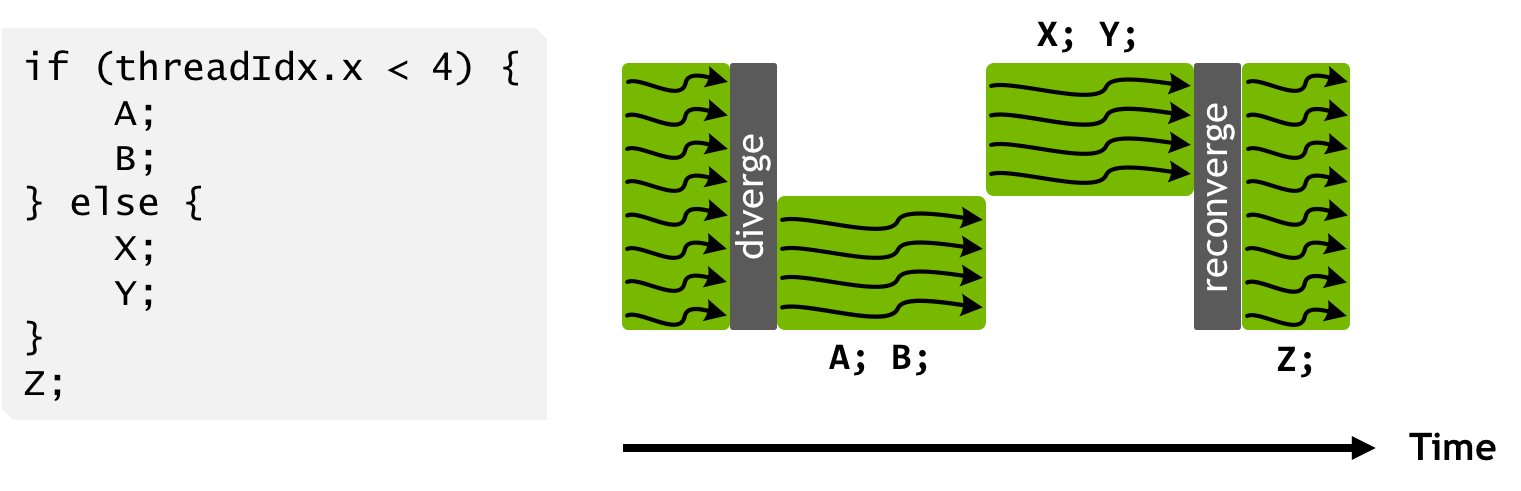
\includegraphics[width=0.8\textwidth]{cuda_thread_divergence_old.png}
	\caption{Branching in device \citep{site:cuda}.}
	\label{fig:thread_divergence_old}
\end{figure}

% TODO: Maybe mention global memory access

On the surface, the device code is very similar to the host code written for the CPU, and will most likely work correctly if written as if for the CPU. But to maximize performance, one must keep in mind the SIMT model, grouping into warps, thread divergence when branching, coalesced memory accesses etc.

On the other side of the spectrum, the SIMT execution model can be compared to the Single instruction, multiple data (SIMD) execution model, where the number of elements processed by a single instruction is directly exposed in the user code, compared to the SIMT model, where the user code itself describes a behavior of a single thread and the grouping of threads is abstracted by the platform. 

\subsection{Thread hierarchy}

Apart from being grouped into warps, threads on the device are also grouped into Cooperative Thread Arrays (CTA), also known as thread blocks. Thread blocks can be one-dimensional, two-dimensional or three-dimensional, which provides an easy way for work distribution when processing arrays, matrices or volumes. Thread blocks are further organized into one-dimensional, two-dimensional or three-dimensional grid, as can be seen in Figure \ref{fig:thread_hierarchy}. When launching a kernel, we specify thread block size and grid size, which combined together give us the number of threads executing the given kernel.

\begin{figure}[h]
	\centering
	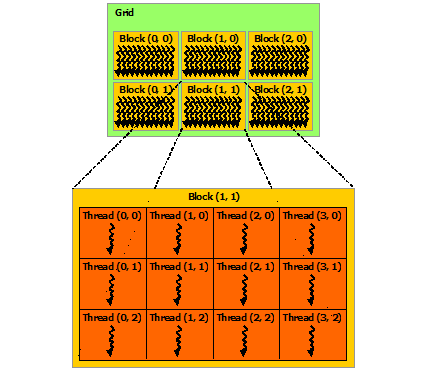
\includegraphics[width=0.8\textwidth]{grid_of_thread_blocks.png}
	\caption{Thread grouping hierarchy \citep{site:cuda}.}
	\label{fig:thread_hierarchy}
\end{figure}

Each thread is assigned an index, accessible through \texttt{threadIdx} built-in variable. Each thread can also access the index of the thread block it is part of through \texttt{blockIdx}, the block size through \texttt{blockDim} and grid size through \texttt{gridDim}. All of these variables are three dimensional vectors, with dimensions unused during kernel launch set to zero for indices and one for dimensions. Using these built-in variables, we can distribute work between threads, most often assigning each thread a part of the input to process.

\subsection{Thread cooperation}
\label{sec:thread_cooperation}
CUDA provides several mechanisms for thread cooperation. Threads can cooperate on the following levels of thread hierarchy, with increasing speed and capability:

\begin{itemize}
	\item grid level,
	\item thread block level,
	\item warp level.
\end{itemize}

The rest of this subsection describes the older API using intrinsic functions. The newer Cooperative Groups API, which is a superset of the older API, is described in the subsection \ref{sec:cooperative_groups}.

\subsubsection{Grid level}
On grid level, the only available tools for cooperation are atomic operations on global memory. These operations can be used to perform read-modify-write on a 32-bit or 64-bit word in global memory without introducing race conditions.

\subsubsection{Thread block level}
On a thread block level, threads can use two mechanisms for cooperation:
\begin{itemize}
	\item shared memory,
	\item synchronization barrier.
\end{itemize}

As per the CUDA C++ programming guide: 
"the shared memory is expected to be a low-latency memory near each processor core (much like an L1 cache) and \_\_syncthreads() is expected to be lightweight" \citep{site:cuda}.

Shared memory is a small on-chip memory, described in more detail in the subsection \ref{sec:memory_hierarchy}. Each thread block has private shared memory, accessible only from threads of the given thread block. Shared memory can be used as software managed cache or to share results between threads of the thread block. 

To synchronize access to shared memory between threads of the thread block, we use synchronization barrier \texttt{\_\_syncthreads()}. All threads in the block must execute the call to \texttt{\_\_syncthreads()} before any of the threads can proceed beyond the call to \texttt{\_\_syncthreads()}. 
The \texttt{\_\_syncthreads()} function also serves as memory barrier. % TODO: Maybe describe what memory barrier is

\subsubsection{Warp level}
% TODO: Describe masks for all the functions
On warp level, threads of the warp, or lanes as they are referred to in the documentation, can utilize intrinsic functions to exchange data without the use of shared memory and perform simple hardware accelerated operations. For operations, warps can perform:
\begin{itemize}
	\item reduce-and-broadcast operations,
	\item broadcast-and-compare operations,
	\item reduce operations,
\end{itemize}

% This is important as this is the basis of one of our algorithms
For data exchange, CUDA C++ provides several warp shuffle instructions. There are four source-lane addressing modes:
\begin{itemize}
	\item direct lane index,
	\item copy from lane with ID lower by \textit{delta},
	\item copy from lane with ID higher by \textit{delta},
	\item copy from lane based on bitwise XOR of provided \textit{laneMask} and own lane ID. 
\end{itemize}

The data exchange does not have to span the whole warp. Shuffle operations allow the warp to be subdivided into groups with width of any power of 2.

Only direct lane indexing performs lane index wrap around. If the given lane index is out of the range $[0:width - 1]$, the actual lane index is computed as $srcLane \mod width$. In other addressing modes, the lanes with out of range source lane index are left unchanged, receiving the value they pass in. The wrap around mechanism allows us to rotate data between threads instead of just shifting. The direct lane indexing can also be used to broadcast a value from a single lane to all other lanes. % TODO: Maybe mention how the wrap around can be used to implement ring buffer shifting between two parts of a buffer

For warp level operations, the reduce-and-broadcast operations receive a single integer value from each lane which they compare to zero, making it effectively a boolean. The results of the comparison are then reduced in one of the following ways and the result is broadcast to all threads:
\begin{itemize}
	\item result is non-zero if and only if all of the values are non-zero,
	\item result is non-zero if any of the values are non-zero,
	\item result contains single bit for each lane which is set if the value given by the lane was non-zero
\end{itemize}

The broadcast-and-compare operations broadcast the value given by each lane and compare it to the value given by the current lane, returning:
\begin{itemize}
	\item mask of lanes that have the same value,
	\item mask if all threads in mask gave the same value, 0 otherwise.
\end{itemize}

Finally, there are the general reduce operations. \textit{Add}, \textit{min}, \textit{max} operations are implemented for signed or unsigned integer values. \textit{And}, \textit{or}, \textit{xor} operations are implemented for unsigned integers only.

The API described in this subsection forms the basis of thread cooperation in CUDA. Most of this API is available since the early versions of CUDA. Subsection \ref{sec:cooperative_groups} will describe a newer Cooperative groups API, which builds on top of and extends the API described in this subsection.

\subsection{Cooperative groups}
\label{sec:cooperative_groups}

Cooperative Groups API, introduced with CUDA 9, is an extension to the CUDA programming model for organizing groups of communicating threads \citep{site:cuda}. The API introduces data types representing groups of cooperating threads, be it a warp, a part of a warp, a thread block, a grid or even a multigrid (representing multiple grids each running on a separate device). 


The API distinguishes two types of groups. First are the \textit{implicit groups}, which are present implicitly in each CUDA kernel. These are:

\begin{itemize}
	\item thread block,
	\item grid,
	\item multigrid.
\end{itemize}

The API provides functions for the creation of handles for data types representing the implicit groups. 

The other type are \textit{explicit groups}, which must be explicitly created from one of the implicit groups. 

\begin{itemize}
	\item thread block tile,
	\item coalesced group.
\end{itemize}

Both of these groups represent warp or subwarp size grouping of threads. Thread block tile can be created from a thread block or from other thread block tile, representing a warp or a part of a warp of size of a power of 2. The warp level operations described in the previous subsection \ref{sec:thread_cooperation} are available as methods on this group, with mask and width arguments of the built-in functions implicitly derived from the properties of the group. 

% TODO: Explaing coalesced group


Creating a handle for an implicit group is a collective operation, in which all threads of the group must participate. Creating the group handle in a conditional branch may lead to deadlocks or data corruption. It may also introduce unnecessary synchronization points, limiting concurrency. Similarly to implicit group handle creation, partitioning of groups is a collective operation which must be executed by all threads of the parent group and may introduce synchronization points. It is recommended to create implicit group handles and do all partitioning at the start of the kernel and pass const references throughout the code \cite{site:cuda}.

\subsection{Memory hierarchy}
\label{sec:memory_hierarchy}

Each CUDA device has its own DRAM memory, so called \textit{device memory} or \textit{VRAM} in GPU properties, separate from the host system memory and from the \textit{device memory} of all other devices. Physically, \textit{device memory} can be seen on most GPU boards as DRAM chips separate from the main silicon chip.

Data has to be transferred from or to the \textit{device memory} over the PCI-e bus, either explicitly by calls to \textit{cudaMemcpy} or by mapping parts of host memory to the \textit{device memory} address space using the \textit{Unified Memory} system, which then handles the data transfers in the background automatically.

From the point of view of a CUDA thread, there are several types of memory available, as can be seen on Figure \ref{fig:memory_types}. For this thesis, the main types are:

\begin{itemize}
	\item local memory,
	\item shared memory,
	\item global memory,
	\item registers.
\end{itemize}

\begin{figure}[h]
	\centering
	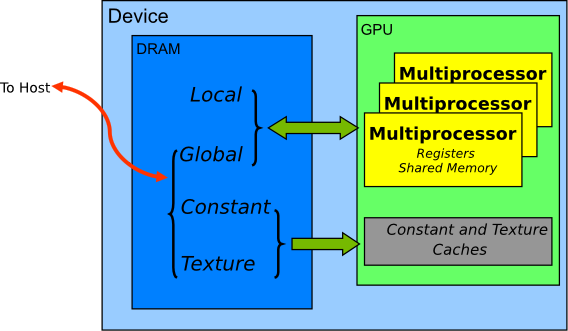
\includegraphics[width=0.8\textwidth]{memory-spaces-on-cuda-device.png}
	\caption{Memory types on a CUDA device \citep{site:cuda}.}
	\label{fig:memory_types}
\end{figure}

Local and global memory are both allocated from device memory, and as such have very high access latency. 

\textbf{Local memory} is private for each thread, allocated automatically based on the requirements of the CUDA compiler. This type of memory is used for register spilling, arrays with non-constant indexing and large structures or arrays which would consume too much register space. 

\textbf{Global memory} is shared by all threads of a kernel, and as such any access which could lead to race condition must be synchronized using atomic operations, as described in Section \ref{sec:thread_cooperation}. Global memory is allocated by the host code using \texttt{cudaMalloc} family of functions. When host code transfers data to the device using \texttt{cudaMemcpy} or any other means, global memory is the part of device memory this data will reside in. The pointers returned by \texttt{cudaMalloc} and possibly used in \texttt{cudaMemcpy} are then passed as arguments to the kernel. Device code can then use these to access the global memory. 

\textbf{Shared memory}, as mentioned in the section \ref{sec:thread_cooperation}, is expected to be a low-latency memory near each processor core (much like an L1 cache). The relation with L1 cache can be seen in the fact that each kernel can configure the proportion between hardware allocated to L1 cache and to Shared memory, which means these memories share the same underlying hardware. Shared memory can be allocated either dynamically by declaring an array type variable with the memory space specifier \texttt{\_\_shared\_\_} and providing the size to be allocated during kernel launch, or statically by defining the variable with static size.


\textbf{Registers} are the fastest memory available. Compared to CPUs, GPUs provide large amount of registers. For all recent GPU generations, the register file provides 65536 32bit registers. 

\subsection{Streaming multiprocessor}
\label{sec:sm}
NVIDIA GPUs are build around an array of \textit{Streaming multiprocessors} (SM). SM of a GPU is similar to a core of a multicore CPU. Each SM has separate execution units, schedulers, register file, shared memory and L1 cache. An example of an SM can be seen in Figure \ref{fig:volta_sm}. Each SM can have multiple schedulers, each scheduling up to one warp per cycle. 

Each thread block is assigned to a single SM exclusively, and each SM can run multiple thread blocks at once. Warps of all thread blocks resident on the given SM are scheduled regardless of the thread block the warps belong to.

% TODO: More

\begin{figure}[h]
	\centering
	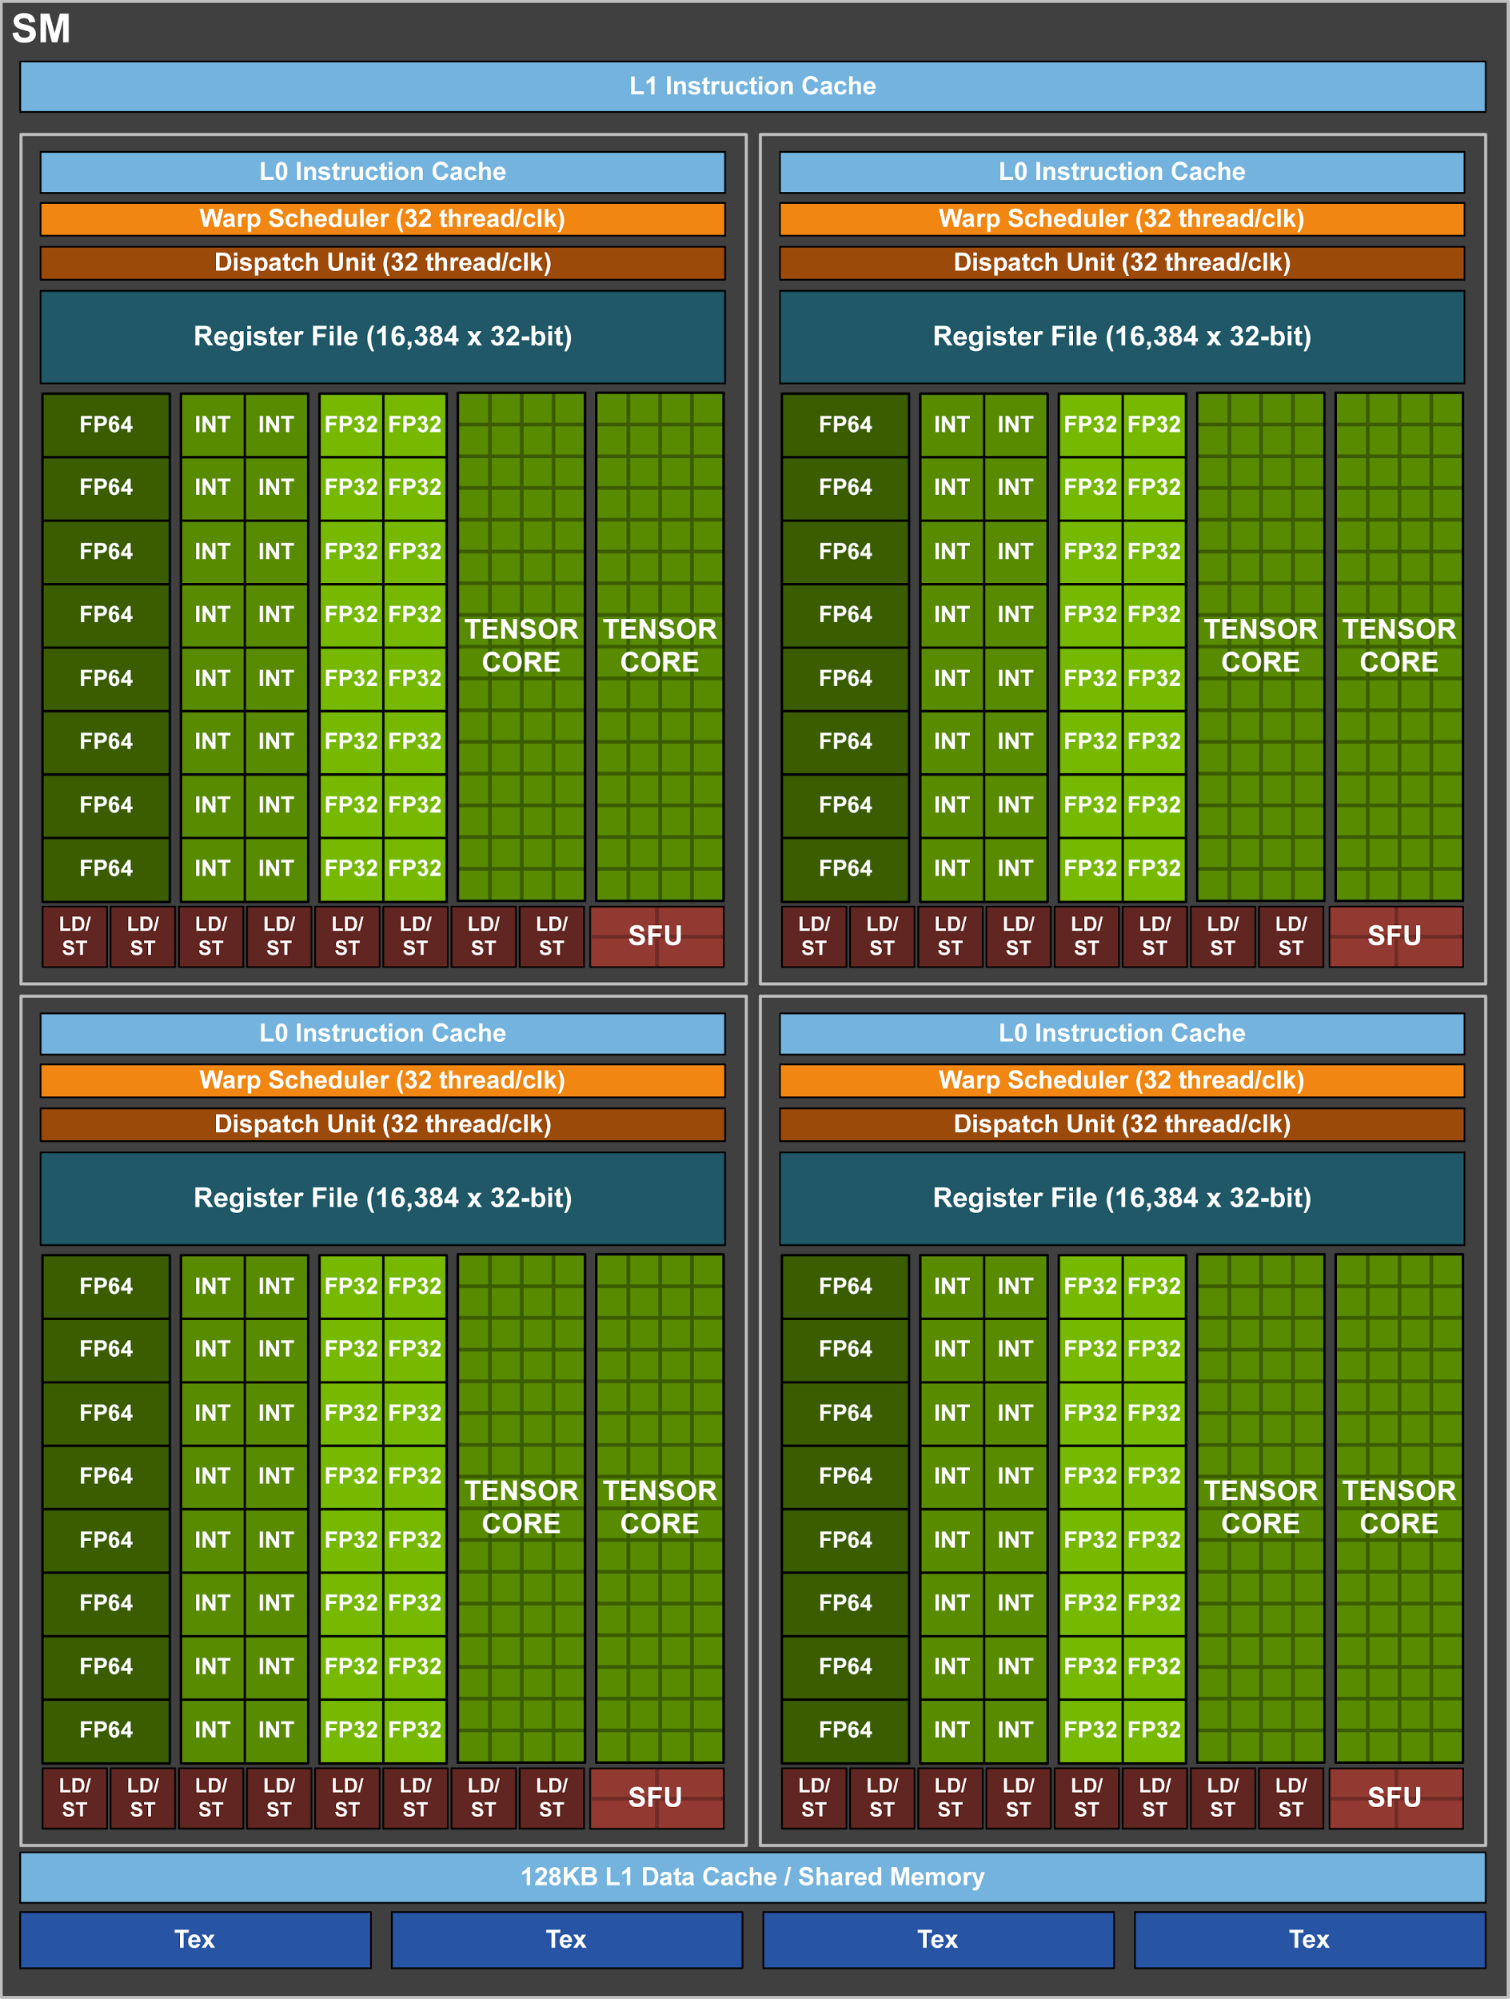
\includegraphics[width=0.8\textwidth]{volta_sm.png}
	\caption{Streaming multiprocessor \citep{paper:volta}.}
	\label{fig:volta_sm}
\end{figure}

\subsection{Versioning}

When working with CUDA, there are two main parts of the platform which are versioned separately: % TODO: Add driver version
\begin{itemize}
	\item CUDA Toolkit,
	\item GPU Compute Capability.
\end{itemize}

CUDA Toolkit represents the software development part of the CUDA platform, encompassing the CUDA runtime library, the \textit{nvcc} compiler and other tools for development of the software.

GPU Compute Capability (CC) represents the features provided by the hardware. This includes the number of registers, memory sizes, set of instructions and other features. In general, each consumer GPU generation corresponds to a new CC, such as GTX 1000 cards corresponding to CC 6.0 Pascal and RTX 3000 cards corresponding to CC 8.0 Ampere. There are some exceptions, for example CC 7.0 Volta having only enterprise cards. With each release of new Compute Capability cards, there is generally accompanying CUDA Toolkit release providing access to the new features provided by the hardware. Compute Capabilities are backwards compatible, so code created for older generation of cards can be ran on newer cards, even though it may not take advantage of new hardware features and may be inefficient on the newer cards.

\section{Code optimizations}

This section introduces basic principles for producing performant CUDA code.
The observations and recommendations provided in this section are based on the principles and properties described in the previous section \ref{sec:programming_model}.

\subsection{Occupancy}

The GPU design prioritizes high instruction throughput of many concurrent threads over single thread performance at the cost of high latency of each instruction. To hide the high latency between dependent instructions, each scheduler keeps a pool of warps between which it switches, possibly on each instruction. Warps in a pool of a scheduler are called \textit{active} warps.
Each cycle, there may be multiple warps which have instructions ready to be executed. Such warps are called \textit{eligible} warps.
Each cycle, a warp scheduler can select one of the \textit{eligible} warps as \textit{issued} warp, issuing its instruction to be executed.

For optimal performance, we want to have enough active warps so that there is at least one eligible warp each cycle to enable the GPU to hide the high latency of each instruction. As described in Section \ref{sec:sm}, the number of warps resident on a SM depends on the number and size of thread blocks resident on a SM.

The number of thread blocks assigned to an SM is limited by three factors:

\begin{itemize}
	\item hardware limit,
	\item register usage,
	\item shared memory usage.
\end{itemize}

The hardware limit differs, but is either 16 or 32 for all currently supported Compute Capabilities. 

To enable no cost execution context (program counters, registers, etc.) switching, the whole execution context for all warps is kept on-chip for the whole lifetime of each warp. 


Number of registers used by all warps of all blocks which reside on the given SM must be smaller than or equal to the number of registers in the register file. For example, for SM with 65536 registers, code using 64 registers per thread and 512 threads in a block, there can only be two blocks resident on the SM, as $2*512*64 = 65536$. If the code requires only a single register more, only a single block will be resident on each SM.

The total amount of shared memory required by all blocks residing on an SM must be smaller than or equal to the size of shared memory provided by the SM. 

\subsection{Pipeline saturation}

Other than occupancy, there are other possible reasons why no warp may be eligible in a given cycle. Pipeline saturation is one of such reasons. GPU hardware has several pipelines, each implementing a different part of the instruction set. As an example, for the RTX 2060 card, these include:
\begin{itemize}
	\item Load Store Unit (LSU),
	\item Arithmetic Logic Unit (ALU),
	\item Fused Multiply Add/Accumulate (FMA),
	\item Transcendental and Data Type Conversion Unit (XU).
\end{itemize}

Each instruction has a Compute Capability specific throughput, which if exceeded makes the pipeline implementing the instruction saturated and unable to execute any other instructions. This becomes a problem when, for example, many or all warps often execute the same low throughput instruction, such as sinus, cosinus or inverse square root, which are implemented by the XU pipeline. Even for simpler operations implemented by the ALU or FMA, if all warps execute the same instruction, the pipelines may become saturated and warps which are waiting to execute more of the given instruction will not be eligible to be issued.

High LSU utilization reflects that the program may be memory bound, waiting for data from global or shared memory, or that the program executes many warp shuffle instructions, which are also implemented by the LSU pipeline. Due to this, the usage of shared memory together with warp shuffles is not advisable, as they both utilize the same pipeline and compete for resources.

% TODO: Maybe screenshot from NSIGHT Compute

\subsection{Global memory access}

As we can see in Figure \ref{fig:global_memory_access}, the access to global memory is grouped into 128~B naturally aligned chunks, where any chunk accessed by any of the threads of the warp has to be transferred from slow global memory. The maximum performance is achieved when access to memory is aligned and coalesced, i.e. all threads of a warp access 32 consecutive 32bit elements of an array which are aligned to 128~B. Any other form of access introduces overhead in a form of unnecessary data being transferred from memory. 

\begin{figure}[h]
	\centering
	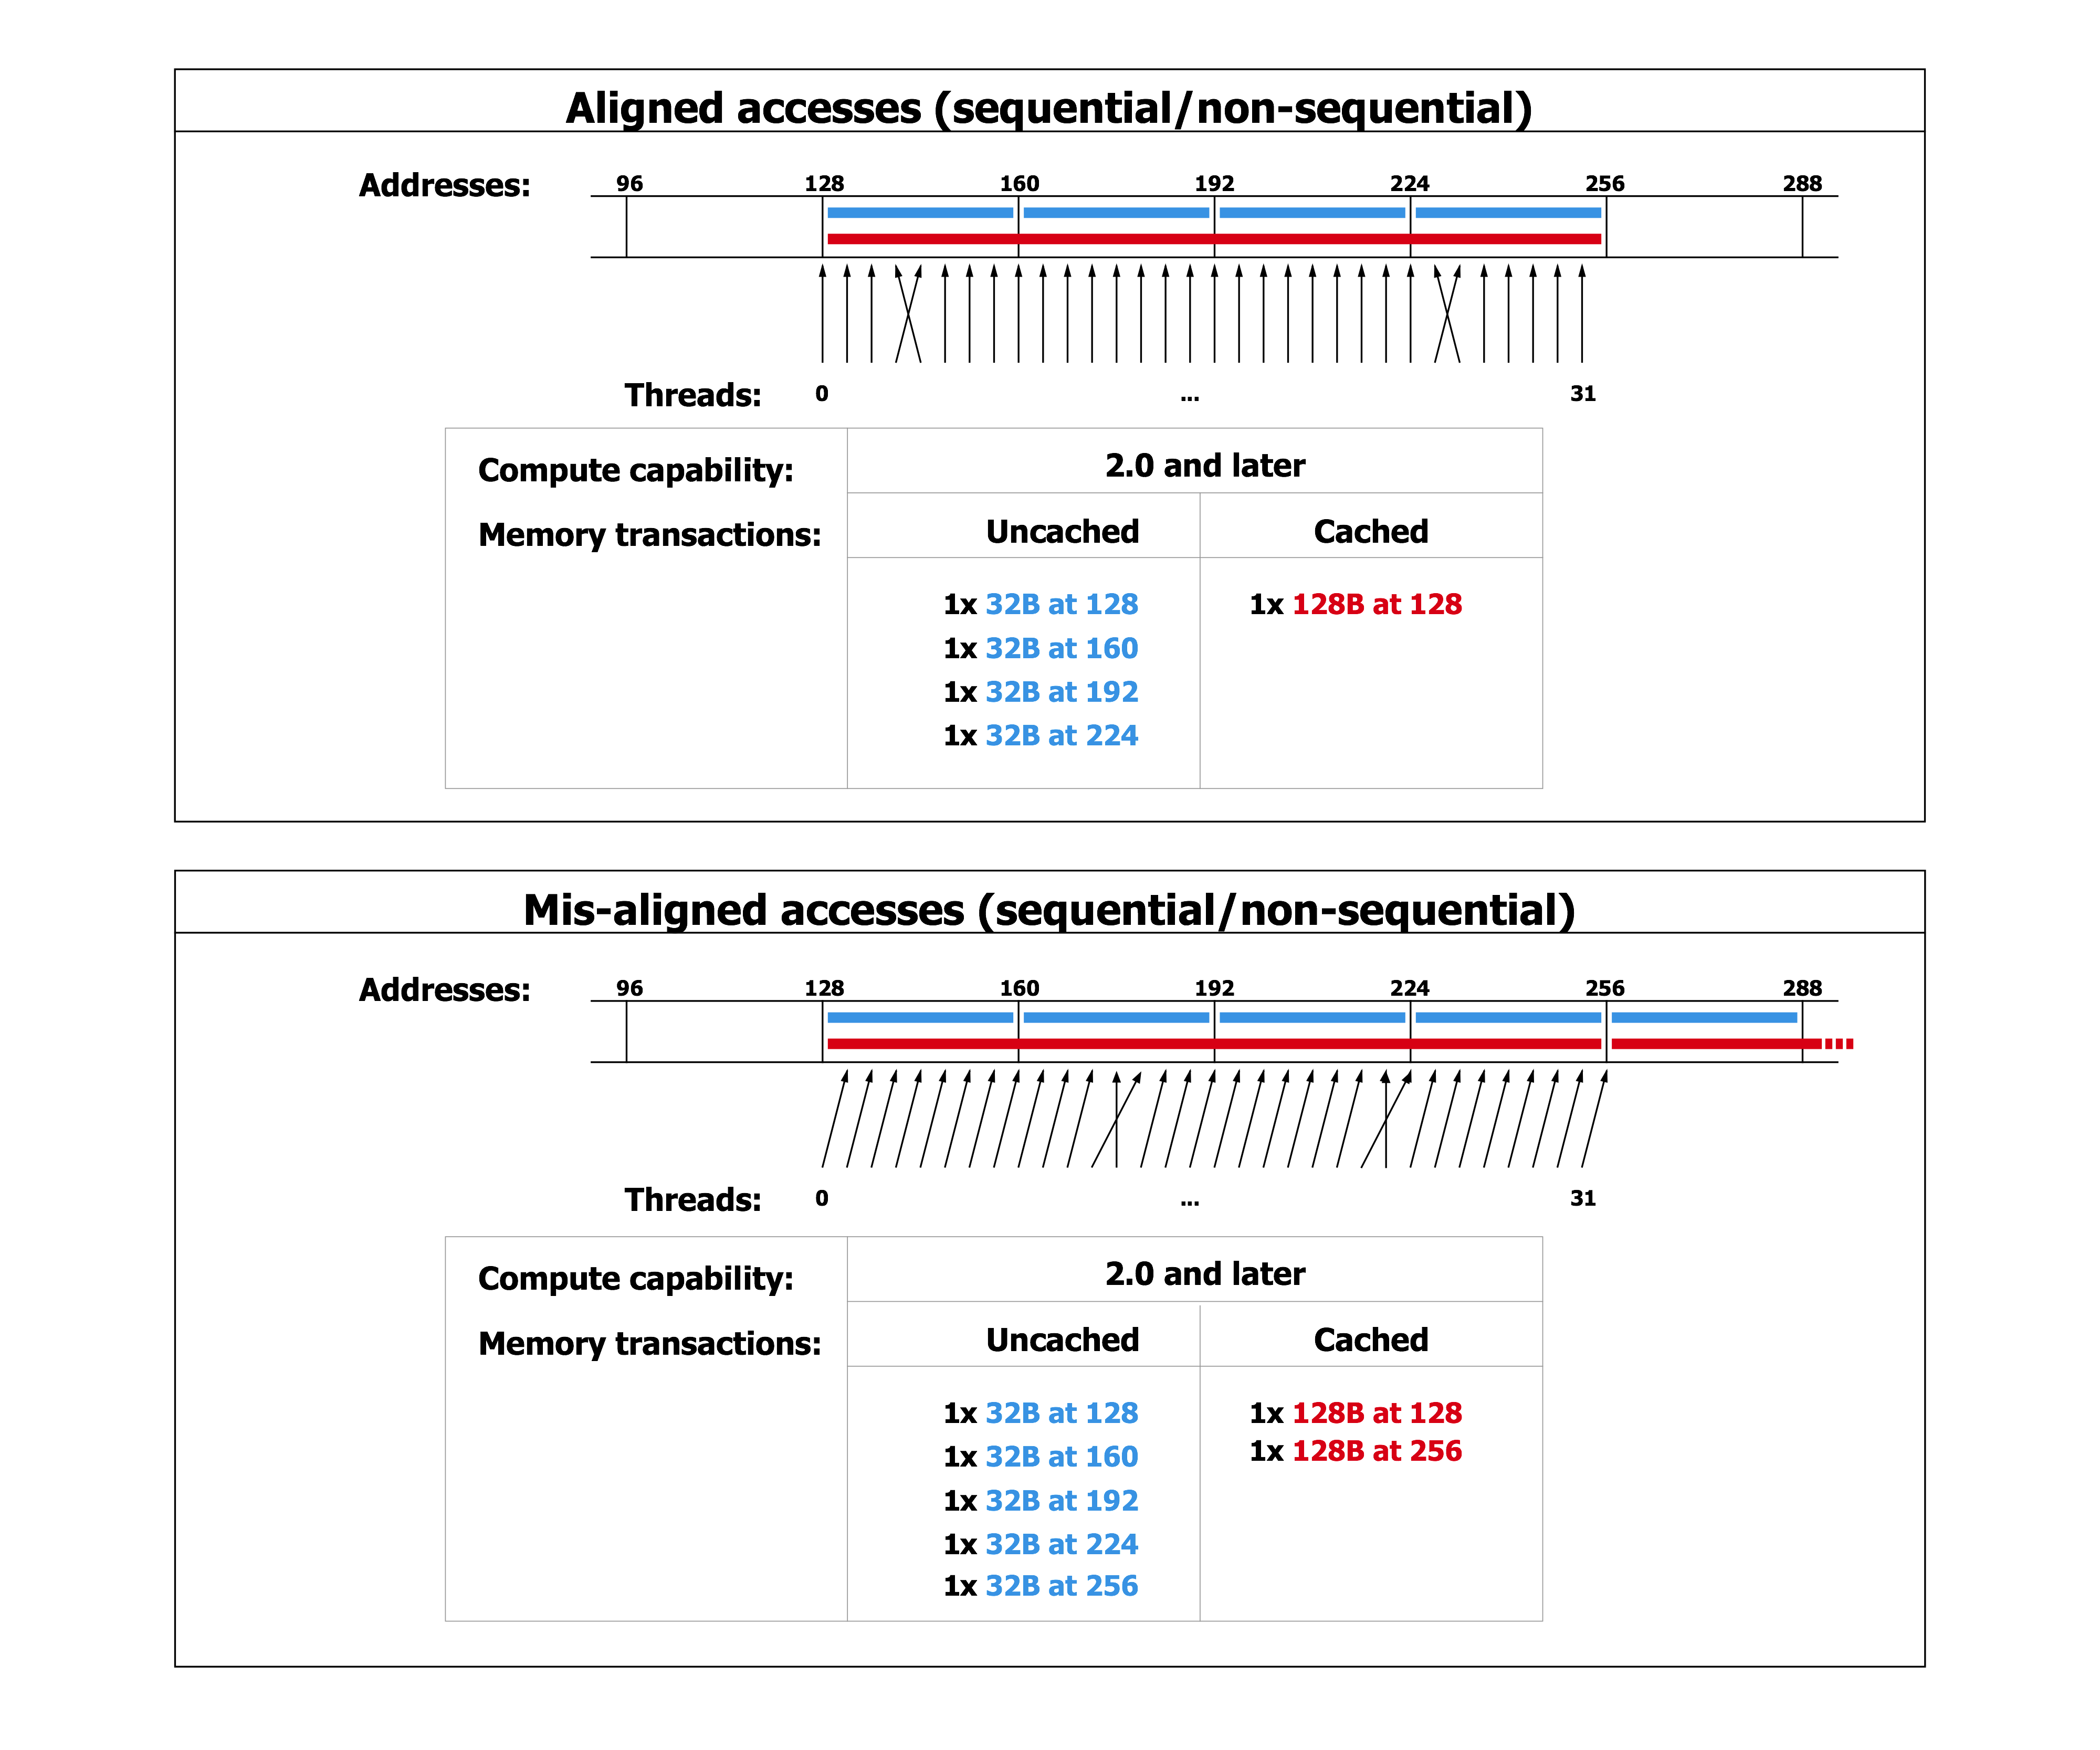
\includegraphics[width=0.8\textwidth]{global-memory-access.png}
	\caption{Global memory access \citep{site:cuda}.}
	\label{fig:global_memory_access}
\end{figure}

\subsection{Shared memory access}
To achieve high bandwidth, shared memory is divided into 32 banks. The optimal access pattern shared memory is designed for is that each thread of a warp accesses a different bank. To enable this access pattern, successive 32bit words are mapped to successive shared memory banks. The simplest pattern is that the 32 threads of a warp access 32 successive 32bit items from an array in shared memory, as can be see in the left column of Figure \ref{fig:shared_memory_access}. If multiple threads access different addresses mapping to the same bank, as can be seen in the middle column of the figure, their accesses are serialized, the throughput being divided by the maximum number of different addresses accessed in any of the banks. This is called a \textit{bank conflict}. Access to a the same address by multiple threads does not lead to a bank conflict, broadcasting the value between the threads instead.

\begin{figure}[h]
	\centering
	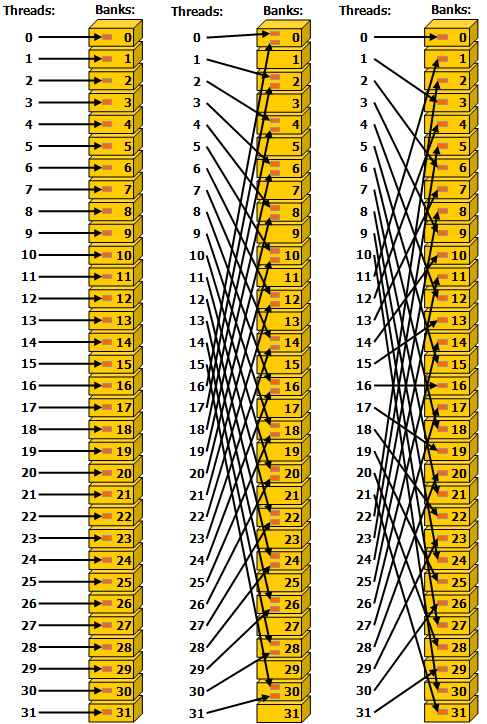
\includegraphics[width=0.8\textwidth]{shared-memory-access.png}
	\caption{Shared memory access patterns \citep{site:cuda}.}
	\label{fig:shared_memory_access}
\end{figure}

\subsection{General recommendations}

We can summarize the information in previous subsections into few simple rules \citep{site:cuda}:

\begin{enumerate}
	\item Maximize parallel execution to achieve maximum utilization;
	\item Optimize memory usage to achieve maximum memory throughput;
	\item Optimize instruction usage to achieve maximum instruction throughput.
\end{enumerate}

To maximize parallel execution, ensure that the workload is distributed between large enough number of threads, where each thread requires low enough number of registers and each thread block requires small enough part of shared memory so that as many as possible fit onto an SM.

To optimize memory usage, minimize transfers from lower bandwidth memory by reusing data in hardware cache or manually move data to shared memory. When accessing global memory, utilize coalesced accesses to minimize unnecessary data transferred. When accessing shared memory, minimize bank conflicts.

To optimize instruction usage, minimize the use of low throughput instructions such as sinus, cosinus or inverse square root. When working with floating point numbers, use 32 bit numbers if precision is not crucial. Minimize thread divergence to ensure all threads in a warp execute useful instructions.

% TODO: Move related work to Analysis chapter
%\section{Related work}

% Accelerating Radio Astronomy Cross-Correlation with Graphics Processing Units

% Kapinchev GPU Implementation of Cross-Correlation for Image Generation in Real Time






\section{Goals}

The goal of this thesis is to measure and quantify the effectiveness of optimizations for different cross-correlation usage patterns. The main objective is to compare the effectiveness of the implementation using Fast Fourier transform and the naive algorithm and measure the input size on which the effectiveness of FFT overtakes the the naive algorithm.

Secondary goal is to optimize the naive implementation from the thesis by \citep{misko}, describe any deficiencies in the original code and quantify the gains when these deficiencies are corrected.

\chapter*{Conclusion}
\addcontentsline{toc}{chapter}{Conclusion}
 
In this thesis, we have analyzed the definition-based cross-correlation algorithm, searching for parallelization and optimization possibilities based on the input matrix size and input type. Based on this analysis, we have implemented two algorithm families, each with many implementations employing different combinations of the optimization and parallelization strategies. The implementations are based on the CUDA framework.

The optimizations target many algorithm properties, from caching and data reuse with the goal of reducing the number of accesses to slower memory types, to the amount of parallelism available to fully saturate the GPU and utilize the full throughput provided by the hardware. Each optimization was rigorously profiled and measured for different input sizes and input types, some trying to optimize across all inputs and some targeting specific combinations of input sizes and types. 

The first algorithm family presented by this thesis was the Warp shuffle family, which utilized warp shuffle instructions to share input data between threads of a warp, significantly reducing the number of accesses to global memory. The family includes further optimizations, which reduce the total number of warp shuffle instructions required. This is achieved by computing cross-correlation between one matrix and many other matrices at once or by computing multiple results from the same cross-correlation at once. Another optimization employed by this family improves parallelization and load balancing.
 
The second algorithm family was the Warp per shift family, which improved occupancy by utilizing a whole warp to compute a single element in the output matrix. This family includes optimizations for data reuse and cooperation of warps through shared memory, together with further improvements to occupancy by utilizing multiple warps per single output matrix element.

We then compared the implementations introduced in this thesis against several other cross-correlation implementations. First, we compared our optimized implementations against a Basic definition-based CUDA implementation. Next, we compared them against an implementation based on the Fast Fourier Transform algorithm also using CUDA. Lastly, we compared our implementations with cross-correlation from production-grade libraries and toolkits, namely with the CPU-based implementation provided by the Python Scipy library and the GPU implementation provided by Matlab. 

When compared with the Basic definition-based CUDA implementation, our optimized implementation achieves at least 5 times speedup for most inputs and up to 10 to 80 times speedup for certain input sizes. When compared with the FFT-based implementation, we achieve speed parity for input matrix sizes over 100x100 for a smaller number of input matrices, decreasing down to 60x60 for a larger number of matrices. In comparison with the CPU-based SciPy library, our implementations achieve 50 times speedup for small input sizes and up to 3000 times speedup for larger input sizes. When compared with Matlab, we achieve around 5 times speedup for small input sizes.
 


\section{Future work}
Although the optimized implementations provided in this thesis are useful and achieve the speedups listed above, they are mostly designed for easy instrumentation and benchmarking. This results in several restrictions on the size and form of the input data, long build times, and a giant executable. In the future, the implementation could be streamlined and the limitations removed.

This thesis also focused heavily on utilizing the CUDA platform for the implementation of the optimized definition-based algorithms. Future work could be aimed at an implementation using other, currently less common tools such as OpenCL. 

Next, the implementations in this thesis utilize only a single GPU. In the future, the implementation could be expanded to utilize more GPUs on a single system or even further to utilize GPUs over multiple systems. Based on the inherent parallelism in the definition-based cross-correlation described in this thesis, the implementation of a distributed version could build on the work provided in this thesis very easily.

To further speed up the definition-based cross-correlation, additional properties of the input data could be used. This includes utilizing non-negative input data and terminating the parts of the computation which cannot reach the current maximum or computing a submatrix of the full cross-correlation matrix.

%%% Bibliography
%%% Bibliography (literature used as a source)
%%%
%%% We employ bibTeX to construct the bibliography. It processes
%%% citations in the text (e.g., the \cite{...} macro) and looks up
%%% relevant entries in the bibliography.bib file.
%%%
%%% The \bibliographystyle command selects, which style will be used
%%% for references from the text. The argument in curly brackets is
%%% the name of the corresponding style file (*.bst). Both styles
%%% mentioned in this template are included in LaTeX distributions.

\bibliographystyle{plainnat}    %% Author (year)
% \bibliographystyle{unsrt}     %% [number]

\renewcommand{\bibname}{Bibliography}

%%% Generate the bibliography. Beware that if you cited no works,
%%% the empty list will be omitted completely.

\bibliography{bibliography}

%%% If case you prefer to write the bibliography manually (without bibTeX),
%%% you can use the following. Please follow the ISO 690 standard and
%%% citation conventions of your field of research.

% \begin{thebibliography}{99}
%
% \bibitem{lamport94}
%   {\sc Lamport,} Leslie.
%   \emph{\LaTeX: A Document Preparation System}.
%   2nd edition.
%   Massachusetts: Addison Wesley, 1994.
%   ISBN 0-201-52983-1.
%
% \end{thebibliography}


%%% Figures used in the thesis (consider if this is needed)
%\listoffigures

%%% Tables used in the thesis (consider if this is needed)
%%% In mathematical theses, it could be better to move the list of tables to the beginning of the thesis.
%\listoftables

%%% Abbreviations used in the thesis, if any, including their explanation
%%% In mathematical theses, it could be better to move the list of abbreviations to the beginning of the thesis.
%\chapwithtoc{List of Abbreviations}

%%% Attachments to the master thesis, if any. Each attachment must be
%%% referred to at least once from the text of the thesis. Attachments
%%% are numbered.
%%%
%%% The printed version should preferably contain attachments, which can be
%%% read (additional tables and charts, supplementary text, examples of
%%% program output, etc.). The electronic version is more suited for attachments
%%% which will likely be used in an electronic form rather than read (program
%%% source code, data files, interactive charts, etc.). Electronic attachments
%%% should be uploaded to SIS and optionally also included in the thesis on a~CD/DVD.
%%% Allowed file formats are specified in provision of the rector no. 72/2017.
\appendix
\chapter{Attachments}

\section{First Attachment}

\openright
\end{document}
